\documentclass[11pt,a4paper]{article}

% --- Packages ---
\usepackage[margin=2.5cm]{geometry}
\usepackage{amsmath,amssymb}
\usepackage{booktabs}
\usepackage{graphicx}
\usepackage{listings}
\usepackage{xcolor}
\usepackage{hyperref}
\usepackage[backend=biber,style=numeric,sorting=none,date=long,urldate=long]{biblatex}
\renewcommand*{\bibfont}{\small}
\addbibresource{refs.bib}
\usepackage{caption}
\usepackage{subcaption}
\usepackage{float}
\usepackage{tikz}
\usetikzlibrary{positioning}
\usepackage{longtable}
\usepackage{array}

% Code listing style for C++ / GLSL / OpenGL
\lstset{
  basicstyle=\ttfamily\small,
  keywordstyle=\color{blue}\bfseries,
  commentstyle=\color{gray},
  stringstyle=\color{red!70!black},
  numbers=left,
  numberstyle=\tiny\color{gray},
  numbersep=5pt,
  frame=single,
  breaklines=true,
  tabsize=4,
  showstringspaces=false,
  language=C++
}

\title{IN3005 Computer Graphics Coursework\\[0.3em]
       \large Tactical Escape game based off \emph{The Quantum Thief}}
\author{Anker Rasmussen \\ 230022888}
\date{\today}

\begin{document}
\maketitle

% ======================================================================
\section{Overview}
% ======================================================================

I made a 3D OpenGL scene and game based on the \textit{Quantum Thief}
trilogy by Hannu Rajaniemi~\cite{rajaniemi2010}. You play the
\textbf{Perhonen}, a small solar-sail starship that belongs to the Oortian
warrior Mieli, while she and Jean le Flambeur try to escape a Sobornost
ambush.

The game has two phases:

\begin{itemize}
  \item A scripted\textbf{ bridge cutscene} (\texttt{Game.cpp}) where Jean
        and Mieli talk, a portrait of the \emph{pellegrini} warns about an
        incursion, and the front wall of the bridge goes transparent to
        show the Sobornost fleet outside.
  \item A \textbf{tactical escape phase} (\texttt{TacticalGame.cpp}) where
        the Perhonen flies along a Catmull--Rom spline through enemy fire.
        You plan moves on a 10-lane grid, then watch the ship fly the
        path you planned.
\end{itemize}

The route is built in code and the ship is procedural. Only the characters
and a few background props are loaded as meshes.

\begin{figure}[H]
  \centering
  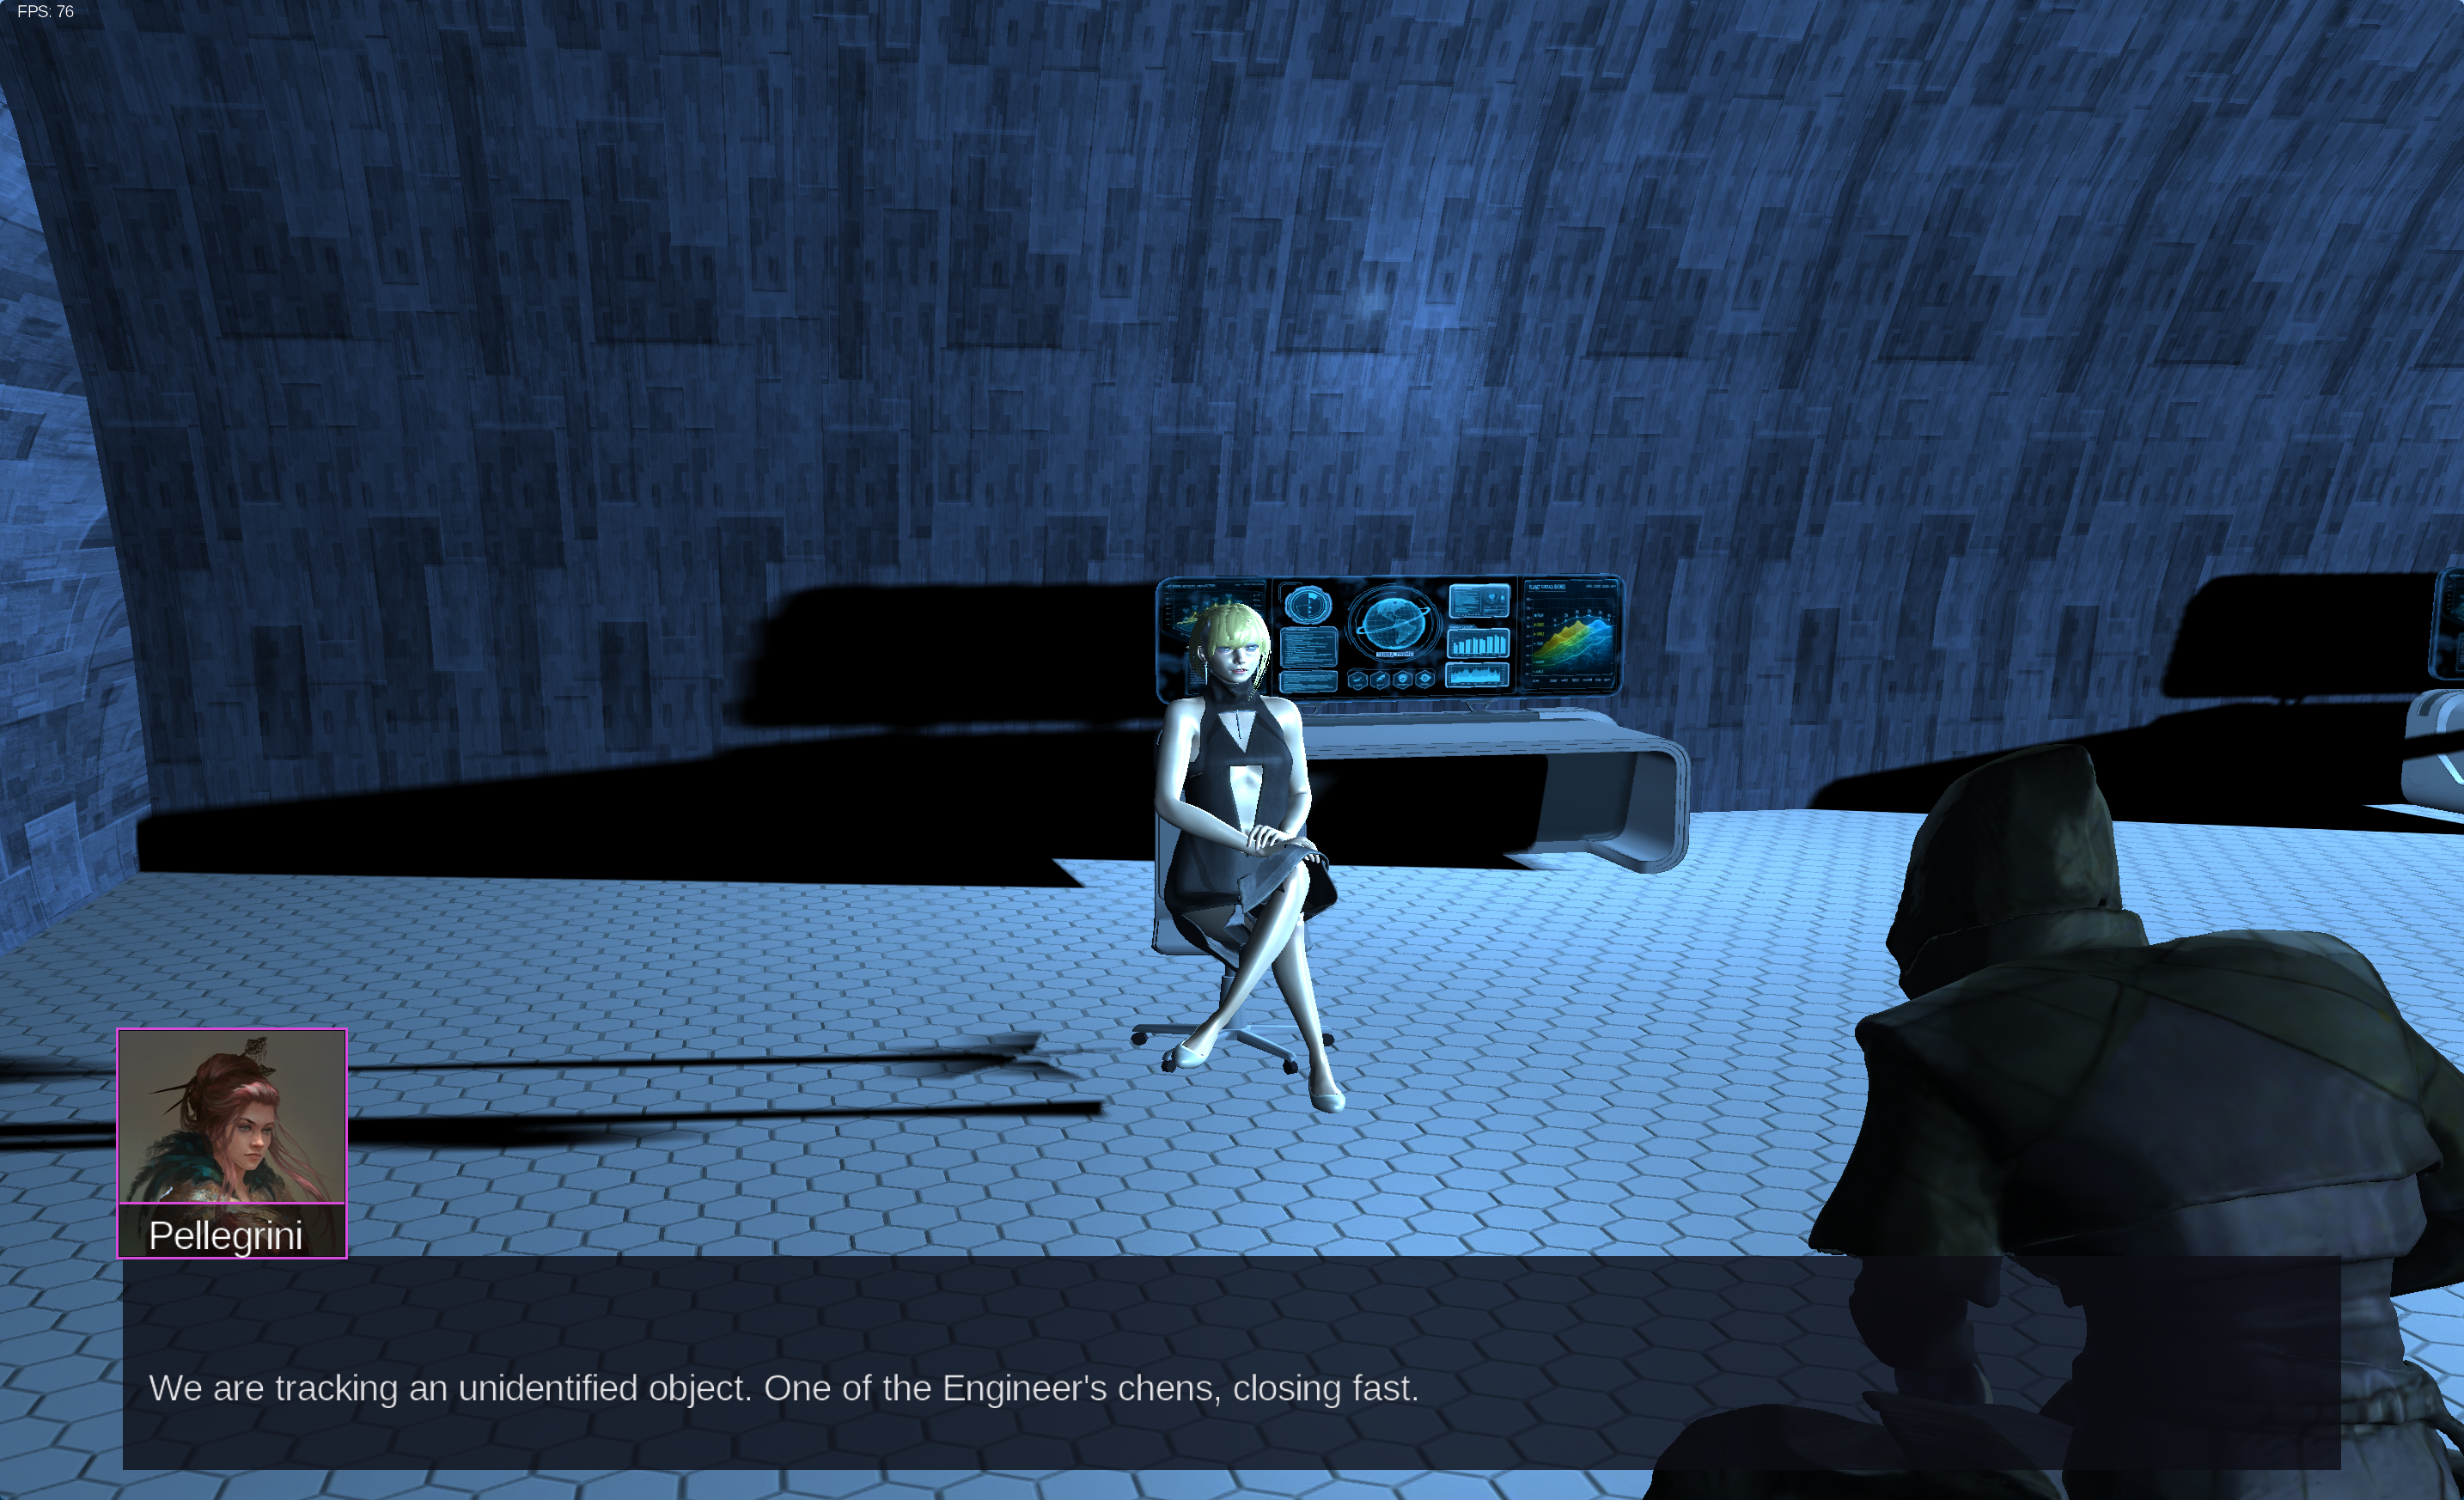
\includegraphics[width=0.6\textwidth]{img/cutscene.jpg}
  \caption{Bridge cutscene: Pellegrini's hologram delivers the incursion
           warning. Dialogue box and portrait nameplate visible bottom-left.}
  \label{fig:bridge}
\end{figure}

\begin{figure}[H]
  \centering
  \begin{tikzpicture}
    \node[anchor=south west, inner sep=0] (img) at (0,0)
      {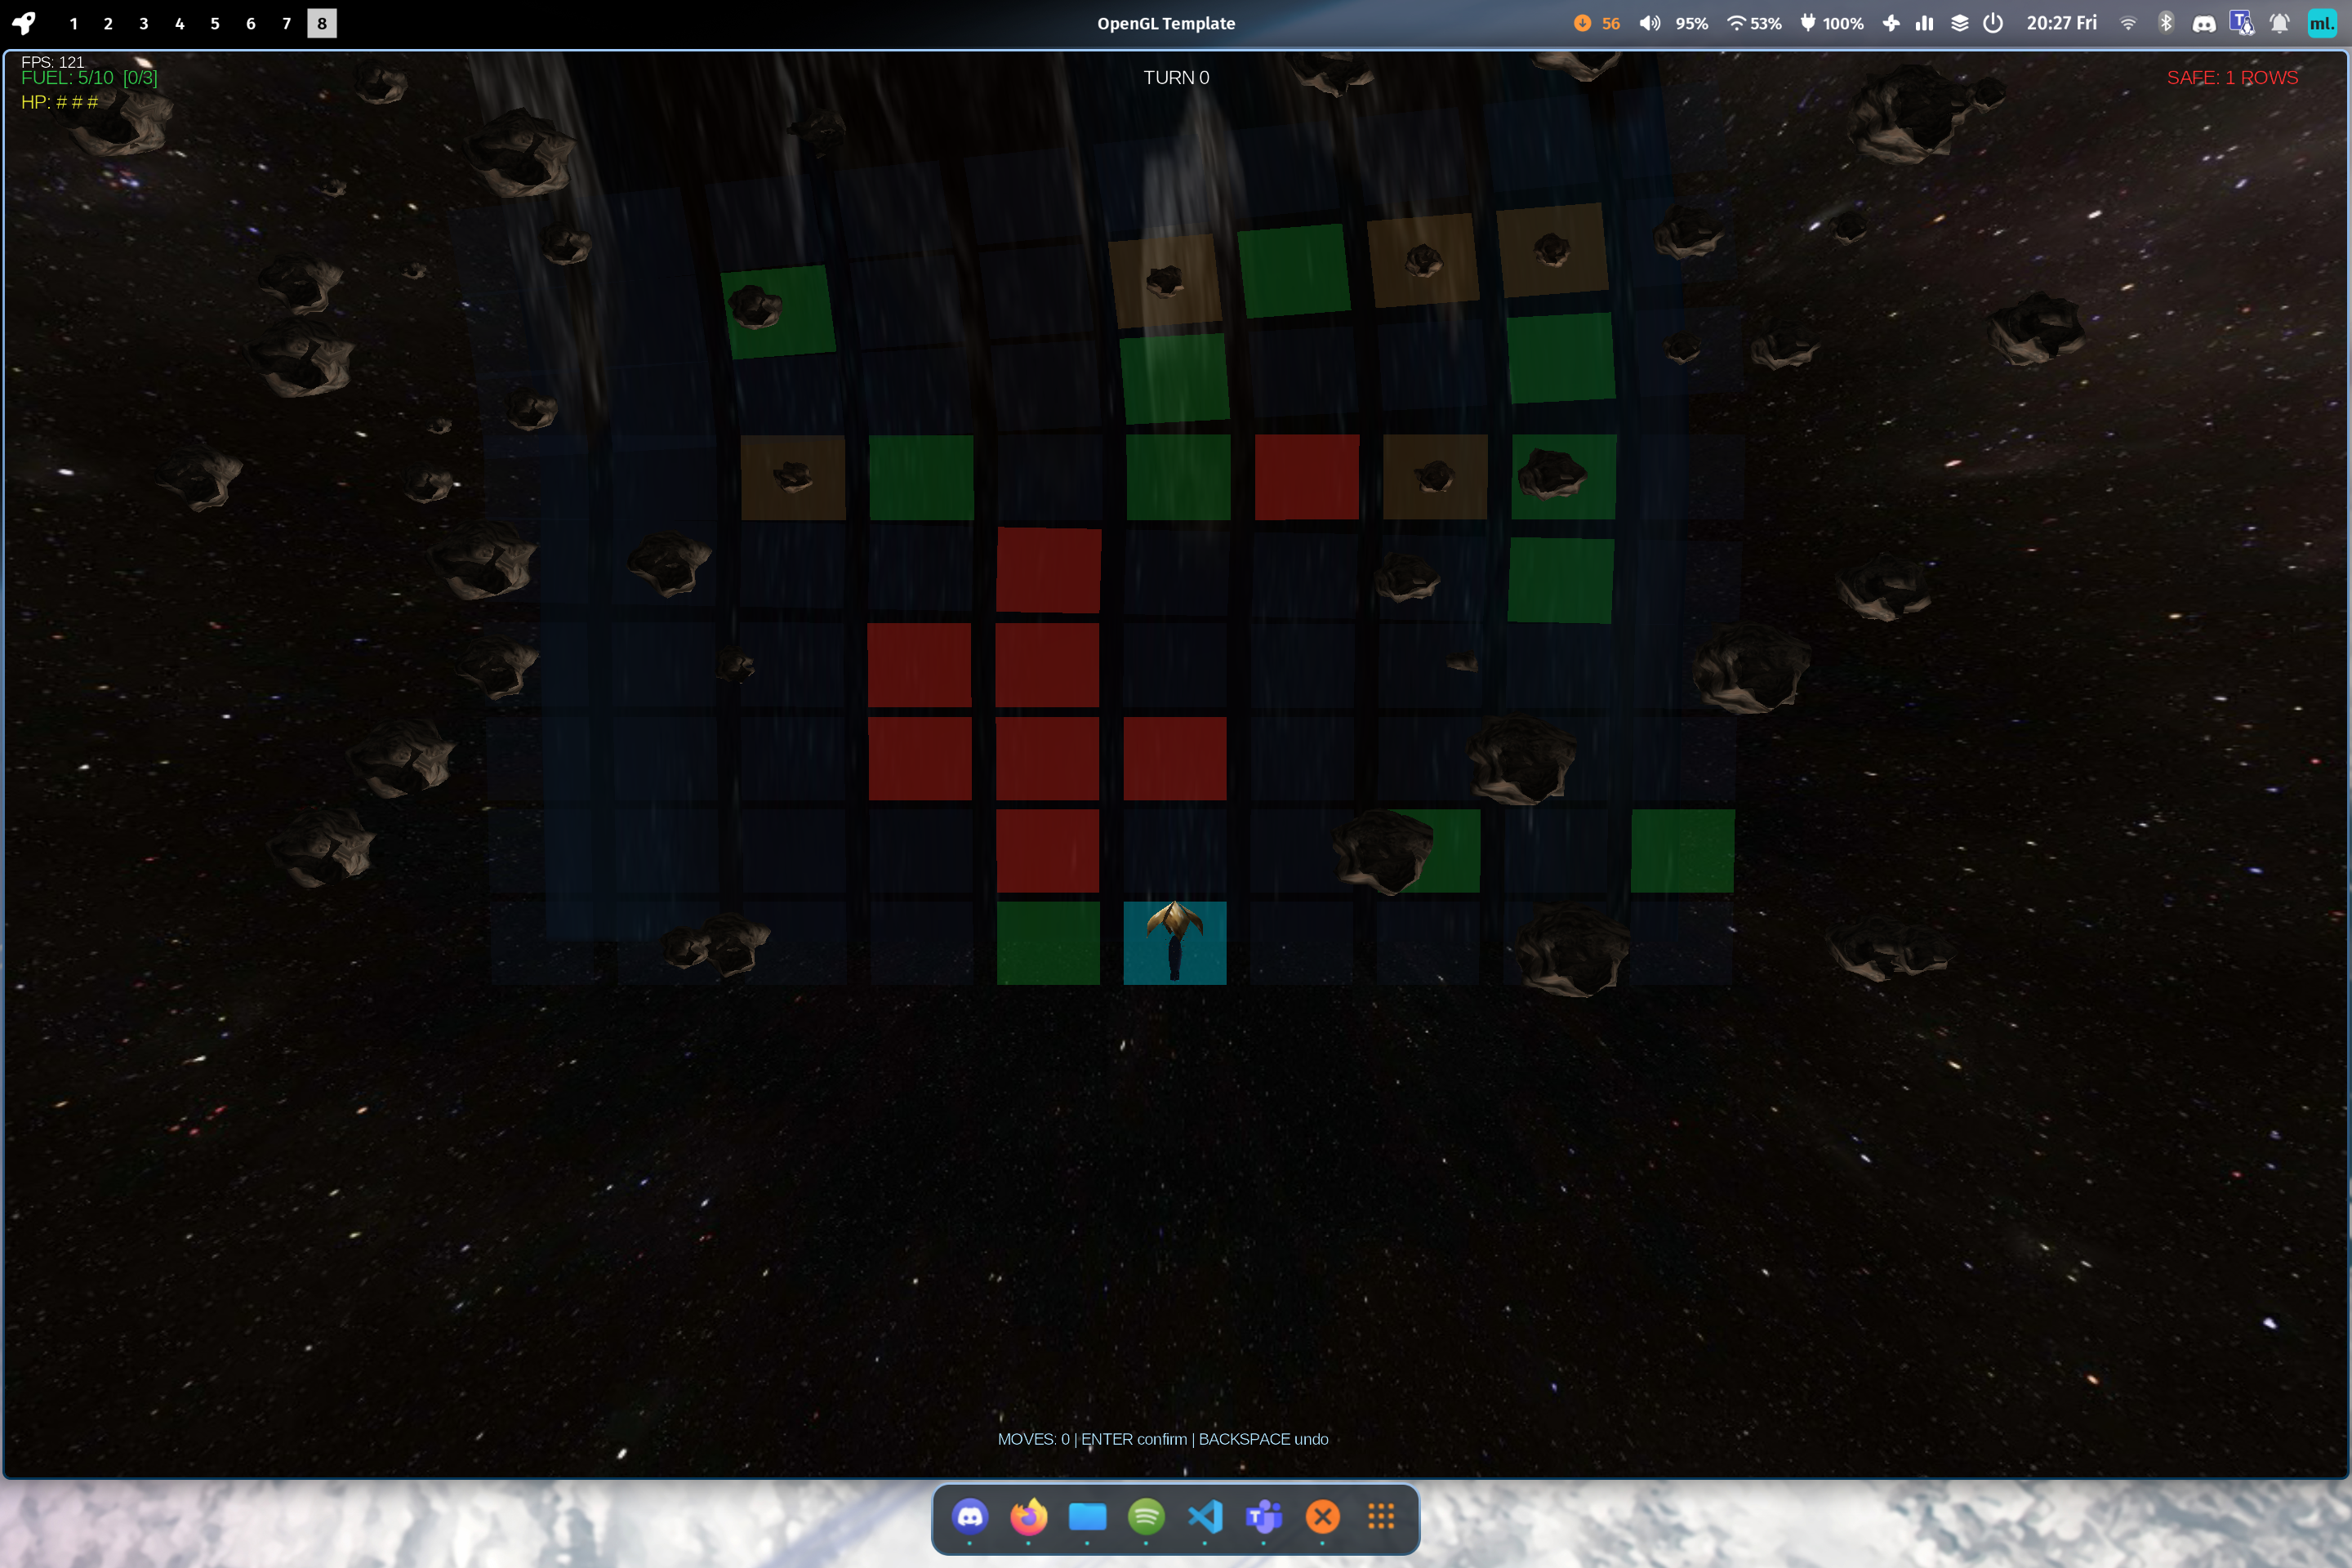
\includegraphics[width=\textwidth]{img/tactical_overview.jpg}};
    \begin{scope}[x={(img.south east)},y={(img.north west)}]
      \tikzset{lbl/.style={fill=white,fill opacity=0.92,text opacity=1,
                            inner sep=2pt,font=\footnotesize\sffamily,
                            rounded corners=1pt,draw=black,line width=0.2pt}}
      \tikzset{cb/.style={-latex,line width=0.6pt,draw=yellow!90!black}}
      % Player ship
      \draw[cb] (0.66,0.16) -- (0.51,0.34);
      \node[lbl] at (0.74,0.13) {Player ship (Perhonen)};
      % Danger cell (red)
      \draw[cb] (0.16,0.55) -- (0.42,0.52);
      \node[lbl] at (0.10,0.55) {Danger cell};
      % Fuel pickup (green)
      \draw[cb] (0.16,0.78) -- (0.34,0.77);
      \node[lbl] at (0.10,0.78) {Fuel pickup};
      % Asteroid obstacle (brown)
      \draw[cb] (0.92,0.71) -- (0.62,0.68);
      \node[lbl] at (0.92,0.74) {Asteroid obstacle};
      % Off-grid scenery asteroid
      \draw[cb] (0.22,0.20) -- (0.08,0.48);
      \node[lbl] at (0.27,0.18) {Off-grid scenery asteroid};
      % HP / fuel HUD (top-left)
      \draw[cb] (0.20,0.88) -- (0.06,0.94);
      \node[lbl] at (0.27,0.88) {HP / fuel HUD};
      % Moves / turn HUD (bottom)
      \draw[cb] (0.50,0.05) -- (0.50,0.085);
      \node[lbl] at (0.50,0.025) {Moves / turn readout};
    \end{scope}
  \end{tikzpicture}
  \caption{Top-down view during the tactical planning phase, annotated.
           The dark blue cells form the 10-lane grid laid along the
           Catmull--Rom centreline; red cells are danger zones from
           incoming enemy fire; green cells are fuel pickups; brown cells
           are destructible asteroid obstacles. The player ship sits
           centre-bottom; the irregular grey rocks scattered outside the
           grid are off-grid scenery asteroids (cosmetic only). The
           tactical HUD splits across two readouts: HP and fuel
           top-left, moves and turn counter centre-bottom.}
  \label{fig:topdown}
\end{figure}

The route is a Catmull--Rom spline of 15 control points. It does not
loop. The brief specifies a route, not a closed circuit, and an open
spline fits the escape narrative (the player flees outward, never
returning to the start). The function \texttt{CreateCentrelineEscape()}
generates it (\texttt{CatmullRom.cpp:191}). The grid (\texttt{CTacticalGrid}) sits on
top of the spline. Each row is 20 arc-length units along the centreline,
and there are 10 lanes across.

There are two kinds of asteroid in the tactical phase.
\textbf{On-grid obstacles} (\texttt{CellType::Asteroid}) are destructible,
sit on a fixed \texttt{(row, lane)} cell, and cost two fuel to push
through. \textbf{Off-grid scenery} asteroids float around freely and are
just for looks. Enemy
ships aren't gameplay objects on the grid. Their threat shows up as
``danger'' cells that \texttt{PlaceDangerCells()} writes onto the grid
each turn (\texttt{TacticalGame.cpp:404}). They still show up as scenery
during the cutscene fleet shot.

% ======================================================================
\section{User Interface Controls}
% ======================================================================

\begin{center}
\begin{tabular}{lll}
\toprule
\textbf{Key / input} & \textbf{Phase} & \textbf{Action} \\
\midrule
Mouse click (title)             & Title screen        & Start cutscene \\
Mouse click                     & Cutscene dialogue   & Advance dialogue line \\
\texttt{F2}                     & Any                 & Toggle free-look camera (WASD + mouse) \\
\texttt{W}/\texttt{A}/\texttt{S}/\texttt{D}, arrows & Free-look camera & Translate camera \\
Mouse move                      & Free-look camera    & Rotate camera (yaw / pitch) \\
\texttt{F3}                     & Tactical            & Pin top-down camera \\
\texttt{F4}                     & Tactical            & Pin third-person follow camera \\
\texttt{F5}                     & Tactical            & Pin animated chase camera \\
\texttt{F6}                     & Tactical            & Return to auto (phase-based) camera \\
\texttt{TAB}                    & Any                 & Toggle ship mode (cruise / combat) \\
$\uparrow$ / $\downarrow$       & Tactical planning   & Queue move forward / backward \\
$\leftarrow$ / $\rightarrow$    & Tactical planning   & Queue move left / right \\
\texttt{Backspace}              & Tactical planning   & Undo last queued move (refunds 1 fuel) \\
\texttt{Enter} / \texttt{Space} & Tactical planning   & Execute planned moves \\
\texttt{Esc}                    & Any                 & Quit application \\
\bottomrule
\end{tabular}
\end{center}

% ======================================================================
\section{Route and Camera}
% ======================================================================

% ----------------------------------------------------------------------
\subsection{Route (15\%)}
% ----------------------------------------------------------------------

The centreline is a Catmull--Rom spline (\texttt{CCatmullRom}). It has $C^1$
continuity~\cite{catmullrom1974}. My function
\texttt{CreateCentrelineEscape()} (\texttt{CatmullRom.cpp:191})
makes a 15-point path in 3D using the standard Catmull--Rom basis matrix.
The lab template's spline is a loop, so I added a non-looping mode
(\texttt{m\_isLoop = false}, \texttt{CatmullRom.cpp:193}) and clamped
sampling at the endpoints. \texttt{SampleTNB()}
(\texttt{CatmullRom.cpp:379}) gives back the tangent / normal /
binormal frame at any distance along the spline. I use it for both the
camera and the grid.

The track itself is rendered as a textured ribbon by
\texttt{CCatmullRom::CreateTrack} / \texttt{RenderTrack}
(\texttt{CatmullRom.cpp:292,409}). I use
\texttt{asteroids.jpg} as the surface texture and lay the UVs along the
spline so the texture wraps continuously down the route. Normals point
along the binormal and lighting uses the standard Phong shader
(\texttt{mainShader.frag}).

Sitting on top of the textured ribbon, I render a separate
\texttt{CTacticalGrid} overlay that shows the playable cells. Each row
is a quad mesh lined up with the spline's TNB frame
(\texttt{TacticalGrid.cpp:252}), drawn untextured with a colour per
cell type (clear, asteroid, danger, pickup, consumed) so the gameplay
state reads at a glance over the textured route below it.


% ----------------------------------------------------------------------
\subsection{Camera (10\%)}
% ----------------------------------------------------------------------

I kept the template's free-view camera. \texttt{F2} toggles it on and off at
any time. On top of that I added camera modes that switch automatically
depending on the game phase. They all use TNB frames sampled from the spline
(\texttt{CTacticalGame::UpdateCamera}, \texttt{TacticalGame.cpp:640}):

\begin{itemize}
  \item \textbf{Top-down view}: used during the \emph{Planning} phase.
        Camera placed at
        $\mathrm{gridCentre} + \mathbf{B}\cdot 350 + \mathbf{T}\cdot 20$,
        looking along $-\mathbf{B}$ with up-vector $\mathbf{T}$
        (\texttt{TacticalGame.cpp:666}).
  \item \textbf{Third-person follow}: the default tactical view. Camera sits
        behind the ship at
        $\mathrm{shipPos} - \mathbf{T}\cdot 45 + \mathbf{B}\cdot 20$ looking
        along $+\mathbf{T}$ (\texttt{TacticalGame.cpp:680}).
  \item \textbf{Animated chase}: used during the \emph{Animating} phase. The
        camera follows the ship's Catmull--Rom path through the planned
        waypoints by calling \texttt{SamplePathCatmullRom} every frame
        (\texttt{TacticalGame.cpp:673}).
  \item \textbf{Cinematic angles}: the cutscene uses fixed angles I picked
        for each dialogue line (over-the-shoulder, side-on dolly, viewport-
        side). These are switched in the cutscene update block in
        \texttt{Game.cpp}.
\end{itemize}

By default I switch these automatically when the phase changes, because
the right framing depends on what you're doing (top-down to plan, chase
to watch the ship fly). On top of the auto-switching I also bind explicit
overrides: \texttt{F3} pins top-down, \texttt{F4} pins third-person,
\texttt{F5} pins the animated chase, and \texttt{F6} returns to
auto-switching. \texttt{F2} is still there for free-look on top of all
of that.


% ======================================================================
\section{Basic Objects, Meshes, and Lighting}
% ======================================================================

% ----------------------------------------------------------------------
\subsection{Basic Objects (10\%)}
% ----------------------------------------------------------------------

I have four procedural objects on top of the template's plane and sphere:

\begin{enumerate}
  \item \textbf{Ship hull} (\texttt{CShip}, \texttt{Ship.cpp:62}): a
        teardrop surface of revolution. I used the slices/stacks scheme from
        Ahn's procedural-sphere notes~\cite{songho_sphere}. Textured with
        \texttt{neon.png}. I wrote a custom \texttt{hullShader} that adds an
        emissive seam glow when the ship is charging.
  \item \textbf{Solar sails} (\texttt{CShip}, \texttt{Ship.cpp:267}): four
        Coons patches~\cite{farin2002coons} arranged as a tetrahedral sail
        array in front of the hull. A single Coons patch was my interim
        coursework submission; the brief allows interim shapes to count
        here, and I extended it into the four-patch sail array plus the
        unfurl animation for the final. Building the array was easy
        because of the symmetry: I just step through four angles around
        the z-axis (\texttt{sailAngles[]} at \texttt{Ship.cpp:269}) and
        place a copy of the patch at each one.
        \texttt{sailShader.vert} lerps each vertex between a furled
        position (collapsed onto the hull axis) and its deployed position.
        A single \texttt{unfurl} uniform $u\in[0,1]$ drives it. This is the
        standard morph-target pattern~\cite{geeks3d_morphtarget}. I added
        two extras on top so the unfurl looks like cloth, not just a mesh
        that's scaling up:
        \begin{itemize}
          \item \emph{Spars before membrane.} I tag boundary vertices
                (within $0.08$ of the patch edge in $(s,t)$-space) as spars
                and drive them with $\mathrm{sparProgress} = \max(s,t)$, so
                the root end extends before the tip. Interior (membrane)
                vertices follow the same curve but lag by about 15\%, so
                the frame deploys first and then the cloth tightens.
          \item \emph{Slack-cloth sag.} Half-unfurled membrane vertices
                get an extra droop
                $\sin(\pi t_\mathrm{unfurl})\cdot\sin(\pi s)\sin(\pi t)$,
                where $t_\mathrm{unfurl}\in[0,1]$ is the per-vertex deploy
                progress. It peaks halfway through the deploy and goes back
                to zero at the start and end, so the cloth looks slack in
                the middle of the unfurl instead of just stretching out
                rigidly.
        \end{itemize}
        The fragment shader also adds a broad iridescent specular term
        using \texttt{iridescent.png}.
  \item \textbf{Asteroids} (\texttt{CAsteroid},
        \texttt{Asteroid.cpp:25,116}): icospheres I displace with 3D Perlin
        noise~\cite{perlin2002}. After the displacement I recompute normals
        and apply a spherical UV. There are two kinds: destructible on-grid
        obstacles and free-floating scenery. Both use \texttt{asteroid.jpg}
        (bound at \texttt{TacticalGame.cpp:103}).
  \item \textbf{Tactical grid} (\texttt{CTacticalGrid},
        \texttt{TacticalGrid.cpp:252}): two triangles per cell that follow the
        spline's TNB frame. Cells are coloured by type (clear, asteroid,
        danger, pickup, consumed). This is the playfield.
\end{enumerate}

All four use texture mapping and Phong lighting.


% ----------------------------------------------------------------------
\subsection{Meshes (10\%)}
% ----------------------------------------------------------------------

I load eight texture-mapped meshes into the scene, on top of the template's
horse and barrel:

\begin{center}
\small
\begin{tabular}{lll}
\toprule
\textbf{Mesh} & \textbf{Purpose} & \textbf{Format / origin}~\footnotemark[1] \\
\midrule
Jean (Mixamo rig)        & Cutscene character      & \texttt{jeansit.fbx} + idle / walking / running / strafe / turn clips \\
Mieli (custom rig)       & Cutscene character      & OBJ rebuilt and rigged via Mixamo, baked atlas \\
Chen                     & Cutscene figure         & \texttt{chen.fbx} + \texttt{Salute.fbx} \\
Cruiser ($\times 3$)     & Sobornost enemy ship    & \texttt{cruiser.glb}, repeated in fleet shot \\
Warmind                  & Sobornost enemy ship    & \texttt{warmind.glb} \\
Monitoring station ($\times 4$) & Bridge prop      & \texttt{Stol2.obj}, repeated \\
Table \& Chair ($\times 2$) & Bridge furniture     & \texttt{TableHall.obj}, \texttt{Chair.obj} \\
\bottomrule
\end{tabular}
\end{center}
\footnotetext[1]{Sources, dates, and licences are listed in
\S\ref{sec:assets}.}

The brief asks for repeated mesh objects in the scene, so I reuse a couple
of meshes: the four monitoring stations on the bridge walls all use the
same station mesh, and the three Guberniya cruisers in the fleet shot are
the same cruiser asset placed at different positions and rotations.


% ----------------------------------------------------------------------
\subsubsection*{Asset pipeline: from base mesh to in-engine FBX}
% ----------------------------------------------------------------------

I downloaded all eight meshes for free from Sketchfab~\cite{sketchfab}, then
ran the character meshes through Mixamo~\cite{mixamo} to auto-rig and
animate them. Both routes end up as FBX or glTF files that Assimp can read.

\begin{description}
  \item[Static glTF / OBJ props.]
        \texttt{cruiser.glb}, \texttt{warmind.glb},
        \texttt{Stol2.obj} (monitoring station),
        \texttt{TableHall.obj}, and \texttt{Chair.obj} are unmodified Sketchfab
        downloads. \texttt{.glb} (binary glTF) packs the mesh, materials,
        and textures into one file, which Assimp reads directly.
        \texttt{.obj}/\texttt{.mtl} pairs ship the texture files alongside
        the geometry.
  \item[Sketchfab mesh re-rigged via Mixamo (Jean, Mieli, Chen).]
        Each character started as a static Sketchfab download with no rig.
        I uploaded the mesh to Mixamo's auto-rigger, placed joint markers
        on the chin, wrists, elbows, knees, and groin, and Mixamo produced
        a skin-weighted FBX with the original mesh bound to Mixamo's
        humanoid skeleton.
        Then I downloaded animation clips from Mixamo's library as separate
        FBX files using the same skeleton (\texttt{idle.fbx},
        \texttt{walking.fbx}, \texttt{running.fbx},
        \texttt{left strafe.fbx}, \texttt{right strafe.fbx},
        \texttt{left/right turn 90.fbx}, \texttt{jeansit.fbx},
        \texttt{sitting talking.fbx}, \texttt{Salute.fbx}).
        Since every clip uses the same bone names, the channels apply to
        each character with no retargeting work in-engine.
  \item[Material consolidation (Mieli).]
        Mieli's download had several material slots, so I ran two Blender
        scripts before rigging to simplify it:
        \begin{itemize}
          \item \texttt{reassign\_materials.py} merged the per-face material
                assignments into a single slot;
          \item \texttt{bake\_atlas.py} baked the per-material textures
                into one atlas (\texttt{mieli\_atlas.png}).
        \end{itemize}
        The resulting FBX uses just one sampler in the shader, so I don't
        need to switch materials at runtime.
\end{description}

So the pipeline is: Sketchfab~$\to$~Mixamo (rig + animations)~$\to$~rigged
FBX + clip FBXs~$\to$~Assimp \texttt{ReadFile}~$\to$~skinning shader. Static
props skip Mixamo and go straight from Sketchfab into Assimp.

% ----------------------------------------------------------------------
\subsubsection*{Mesh loading with Assimp}
% ----------------------------------------------------------------------

All eight meshes are loaded through Assimp~\cite{assimp}. I have two loader
classes that wrap it:

\begin{description}
  \item[\texttt{COpenAssetImportMesh}] (template code, with my fixes) for
        static meshes (\texttt{.glb}, \texttt{.obj}). I load it with
        \texttt{aiProcess\_Triangulate | aiProcess\_GenSmoothNormals |
        aiProcess\_FlipUVs | aiProcess\_PreTransformVertices}. These flags
        force triangle-only faces, generate normals if there aren't any,
        flip the V coordinate (Assimp's default has $+v$ down, OpenGL has
        $+v$ up), and pre-multiply the node hierarchy into the mesh, so
        the \texttt{aiScene} ends up as a flat list of \texttt{aiMesh*}.
  \item[\texttt{CAnimatedMesh}] (I wrote this, following the LearnOpenGL
        skeletal-animation tutorial~\cite{learnopengl_skeletal}) for skinned
        meshes (\texttt{.fbx}). I load it with
        \texttt{aiProcess\_Triangulate | aiProcess\_GenSmoothNormals |
        aiProcess\_FlipUVs | aiProcess\_LimitBoneWeights}. I leave out
        \texttt{aiProcess\_PreTransformVertices} on purpose, because that
        would flatten the skeleton. Instead I walk the node hierarchy at
        runtime to get the bone transforms.
        \texttt{aiProcess\_LimitBoneWeights} caps each vertex at four bone
        influences so the data fits in the skinning shader's
        \texttt{ivec4 boneIDs} / \texttt{vec4 boneWeights} attributes.
\end{description}

For static meshes I read vertices straight from
\texttt{paiMesh->mVertices}, \texttt{mNormals}, and
\texttt{mTextureCoords[0]}, and faces from \texttt{mFaces}. Materials come
from \texttt{aiMaterial::GetTexture(aiTextureType\_DIFFUSE, ...)} and the
textures are loaded relative to the FBX's directory.

For skinned meshes I run an extra \texttt{LoadBones()} pass
(\texttt{AnimatedMesh.cpp}) over \texttt{paiMesh->mBones[i]} that builds:
\begin{itemize}
  \item a \texttt{string $\to$ int} map from bone names to indices, so I
        can match the animation channels (which reference bones by name)
        to the right bone at runtime;
  \item a per-vertex weight list. For each \texttt{aiBone} I go through
        its \texttt{mWeights[]} array and keep the four largest
        contributions per affected vertex.
\end{itemize}
I load each animation clip by re-opening the clip's FBX with a fresh
\texttt{Assimp::Importer}, reading \texttt{pScene->mAnimations[0]}, and
storing every \texttt{aiNodeAnim} channel (per-bone position, rotation, and
scale keyframes) keyed by bone name. At render time
\texttt{ReadNodeHierarchy()} (\texttt{AnimatedMesh.cpp:572}) walks the
hierarchy, samples each channel at the current play time, multiplies each
bone's local transform up its parent chain, and uploads the resulting
\texttt{mat4[MAX\_BONES]} array as a uniform that
\texttt{skinningShader.vert} reads. The function starts at
\texttt{AnimatedMesh.cpp:572}.

\begin{lstlisting}[caption={Assimp import (animated path): core call}]
m_pScene = m_importer.ReadFile(filename.c_str(),
    aiProcess_Triangulate | aiProcess_GenSmoothNormals |
    aiProcess_FlipUVs    | aiProcess_LimitBoneWeights);
// ... walk pScene->mMeshes, mBones, mAnimations
\end{lstlisting}

\paragraph{Robustness patches to \texttt{OpenAssetImportMesh.cpp}.}
I made three small fixes to the static loader so it survives imperfect glTF
assets in the wild:
\begin{itemize}
  \item Null-safe normals: if \texttt{paiMesh->HasNormals()} is false the
        loader falls back to a zero vector instead of dereferencing
        \texttt{mNormals}. Without this, the loader used to crash on
        assets that had no normal channel.
  \item Non-triangle face skip: after \texttt{aiProcess\_Triangulate}, any
        face still reporting \texttt{mNumIndices != 3} (degenerate or
        line-only sub-meshes) is skipped instead of asserting.
  \item Empty-index guard: if a sub-mesh has zero indices (some Sketchfab
        downloads ship with placeholder empty nodes) I skip the VBO bind,
        avoiding a draw call with a zero-size element buffer.
\end{itemize}

% ----------------------------------------------------------------------
\subsection{Lighting (10\%)}
% ----------------------------------------------------------------------

\texttt{mainShader.frag} has a directional sun (\texttt{light1}) and an
array of point lights (\texttt{pointLights[MAX\_POINT\_LIGHTS]}). Right now
the point lights are four dim blue console lights on the bridge, set up at
\texttt{Game.cpp:1356}. Both go through a shared \texttt{PhongModel}
function with attenuation. There's also a spotlight that does not
illuminate independently. It renders to a depth FBO so its shadow
mask modulates the point lights, picking out the viewport area in
shadow rather than washing it in extra light. All the lights are
dynamic: I position the console lights every frame relative to the
bridge (\texttt{Game.cpp:1356--1369}), and the sun direction updates
every frame in exterior scenes.

For shadows, I do two depth-only render passes
(\texttt{Game::RenderShadowMap}, \texttt{Game.cpp:701}) into two FBOs (one
for the sun, one for the spotlight), then sample them in the fragment
shader with PCF (\texttt{ComputeShadowFrom} in \texttt{mainShader.frag}).
The whole approach (depth-from-light into an FBO, \texttt{sampler2DShadow}
comparison, PCF kernel) is adapted from de~Vries' shadow-mapping
tutorial~\cite{learnopengl_shadows}. More detail in \S6.3.


% ======================================================================
\section{HUD, Gameplay, and Advanced Rendering}
% ======================================================================

% ----------------------------------------------------------------------
\subsection{HUD (5\%)}
% ----------------------------------------------------------------------

I have two HUDs:

\begin{itemize}
  \item \textbf{Cutscene HUD overlay}: a sprite-sheet animation from
        \texttt{hud\_spritesheet.jpg}, drawn as a fullscreen quad in screen
        space at a fixed framerate (\texttt{Game::RenderEscapeHUD},
        \texttt{Game.cpp:2380}). It plays during phase transitions to mark
        the switch from cutscene to gameplay. \texttt{m\_hudFrameIndex}
        picks the current frame from the sheet, and I draw it with an
        orthographic projection.
  \item \textbf{Tactical HUD}: drawn during gameplay using FreeType text.
        Shows HP, fuel left, current turn, and how many moves are queued.
        A character portrait popup (the Perhonen warning) shows up at the
        end of a turn when the danger row advances.
\end{itemize}


% ----------------------------------------------------------------------
\subsection{Gameplay (5\%)}
% ----------------------------------------------------------------------

It's a turn-based tactical escape game. Input is keyboard: arrow keys to
move, \texttt{Enter}/\texttt{Space} to confirm, \texttt{Backspace} to undo
(input handling in \texttt{TacticalGame.cpp}).

Each turn runs through four phases (\texttt{TurnPhase} enum in
\texttt{TacticalGame.h}):

\begin{enumerate}
  \item \textbf{Planning}: top-down camera; the player queues moves, each
        costing one fuel (or two to push through an asteroid, which destroys
        it). Movement is constrained by grid bounds and by already-consumed
        danger rows.
  \item \textbf{Animating}: the ship flies a Catmull--Rom path through the
        queued waypoints (\texttt{SamplePathCatmullRom},
        \texttt{TacticalGame.cpp:231}). Enemy fire patterns play out at the
        same time, with timing scaled to the distance per tile.
  \item \textbf{EnemyTurn}: I run a collision check. Any planned cell that
        lands on a \texttt{Danger} cell does damage. The bottom row of
        danger cells is consumed and a new danger row advances forward.
  \item \textbf{NextTurn}: fuel +3 (capped at 10), reveal new rows, go back
        to Planning.
\end{enumerate}

Collision detection is grid-based. Each cell has a \texttt{CellType} and a
\texttt{turnsUntilImpact}, and the ship checks every cell on its planned
path during the animation. The player has three HP. On a hit you get a
2- or 3-layer particle explosion, a screen shake
(\texttt{TacticalGame.cpp:327,379}), and an audio cue. Picking up three
fuel pickups restores 1 HP.

The goal is to fly clear of the encounter. The escape spline has a
finite length, and the player wins on the turn they reach the last row
(\texttt{m\_playerRow >= GetTotalRows() - 1}, \texttt{TacticalGame.cpp:355}).
The player loses if their HP hits zero or if the advancing danger row
catches them. There is no turn-count cap: the encounter ends when one
of those three conditions resolves.


% ----------------------------------------------------------------------
\subsection{Advanced Rendering (20\%)}
% ----------------------------------------------------------------------

I have six techniques here, four of them from the ``Harder'' tier.

% --- 6.3.1 ---
\paragraph{Shadow mapping (Harder).}
I do two depth-only render passes (\texttt{Game::RenderShadowMap},
\texttt{Game.cpp:701}). One renders the scene from the sun's point of view
and one from the bridge spotlight's point of view, into separate depth FBOs
(\texttt{m\_shadowMapFBO}, \texttt{m\_spotShadowFBO}). The main shader
samples both with \texttt{sampler2DShadow}, applies a small constant bias,
and combines the two attenuation factors. Skinned meshes use a separate
vertex shader (\texttt{shadowMapSkinned.vert}) that applies the bone
transforms before writing depth~\cite{learnopengl_shadows}. I also switch
culling to \texttt{GL\_FRONT} during the depth pass
(\texttt{Game.cpp:774,794}) to stop peter-panning (a shadow-mapping
artifact where the shadow looks detached from the object that's casting
it, as if the object is floating).

\emph{Known limitation:} shadows on Jean and Mieli are visibly
imperfect — the cast shadow has gaps and stippling that the static props
in the same scene don't show. I believe the cause is on the rigging side
rather than the shadow-mapping side: the Mixamo auto-rig + bone-weight
clamping (\texttt{aiProcess\_LimitBoneWeights}) leaves some vertices
with subtly different transforms in the depth pass than they have in
the colour pass, so the silhouette the shadow map records doesn't quite
match the silhouette the colour pass renders. The bridge meshes share
the same shadow pipeline and shadow correctly, which is what points to
the rig. I don't currently have the know-how on the Mixamo / Assimp
skinning path to track this down within the time budget; the same depth
pre-pass + PCF works correctly on the static props in the same scene,
so I'm reasonably confident the shadow code itself is sound, and the limit is to do with
the models/rigging.


% --- 6.3.2 ---
\paragraph{Environment mapping (Harder).}
I bind the skybox cubemap to texture unit 10 (\texttt{Game.cpp:1321}) and
sample it in the main fragment shader using a reflection vector
$\mathbf{r} = \operatorname{reflect}(\mathbf{v}, \mathbf{n})$. Reflective
surfaces (the bridge viewport, polished hull plates) blend the skybox
sample with the diffuse term at a fixed reflectivity factor. The
space cutscene uses a Milky Way panorama
(\texttt{resources/skyboxes/sky-pano-milkyway/}); the planetary scenes use
a \texttt{jajdarkland1} set.


% --- 6.3.3 ---
\paragraph{Particle animation (Harder).}
\texttt{CParticleSystem} keeps a CPU-side particle pool (position,
velocity, colour, lifetime). They're drawn at
\texttt{ParticleSystem.cpp:232}. I spawn particles with a configurable
cone of initial velocities and render them as point sprites through
\texttt{particleShader}. I use it for asteroid explosions on the tactical
grid (a 3-layer spawn: blood-red, dark-red, orange) and for the Sobornost
warp-in (next paragraph).


% --- 6.3.3b ---
\paragraph{Sobornost warp-in (composite effect).}
The cinematic moment of the cutscene is the ambush: three Guberniya
cruisers and a Warmind drop out of warp around the \emph{Perhonen} on a
staggered timer (\texttt{Game.cpp:2124--2163}). Each arrival is a
composite of four effects layered together rather than a single trick:
\begin{itemize}
  \item \textbf{Two-layer particle burst} per cruiser: 40 cool-white
        particles in a cold core
        $(0.8, 0.85, 1.0)$ and 30 wider warp-blue particles
        $(0.3, 0.5, 1.0)$ flaring behind them. Cruisers emerge close to
        the camera (z\,$\approx$\,100), so I keep particle sizes small
        (4--10 world units) — the world-space sprite size that reads as
        a tasteful flare up close becomes a blown-out blob when reused
        verbatim. The Warmind, by contrast, emerges $\sim$12$\times$
        further out at z\,$\approx$\,1200--1800, so its much larger
        particles (40--100 world units) project to roughly the same
        screen size while letting it use nine spawn sites and four colour
        layers (hot amber-white core, hot-orange bloom, blood-red and
        dark-red outer shrapnel; $\sim$720 particles total) so the
        silhouette of the larger ship still reads against a deep-space
        skybox.
  \item \textbf{Full-screen flash} via the \texttt{m\_screenFlash}
        scalar (warm white at $0.2$ for cruisers, blood-red at $0.85$
        for the Warmind), drawn as an additive fullscreen quad and
        decayed at $-1.5\,\mathrm{s}^{-1}$ (cruisers) or
        $-0.5\,\mathrm{s}^{-1}$ (Warmind). Cruiser flashes are kept
        intentionally subtle so three back-to-back arrivals don't
        whiteout the bridge; the Warmind's red flash latches the
        moment \texttt{m\_shipArrived[3]} flips, which is what
        actually sells the scale shift between the two enemy classes.
  \item \textbf{Camera shake} at the same intensity through the existing
        rotation-based shake system ($s = 0.5$ for cruisers, $s = 1.0$
        for the Warmind), so the bridge feels physically rocked.
  \item \textbf{Audio} (\texttt{warpin.wav}) at the same staggered
        timestamps, with the Warmind's at full volume to sell the scale
        difference.
\end{itemize}
Decay rates were tuned so the Warmind takes roughly three times as long
to settle as a cruiser does, which (along with the extra particle layers)
is the whole reason the Warmind reads as much larger than its mesh
would suggest on its own.


% --- 6.3.4 ---
\paragraph{Skeletal animation / skinning (not listed on spec list).}
\texttt{CAnimatedMesh} (\texttt{AnimatedMesh.cpp}) loads Mixamo FBX rigs
through Assimp, building a bone hierarchy and a list of \texttt{aiNodeAnim}
channels per clip. Every frame I interpolate the bone matrices and upload
them as a uniform array, and \texttt{skinningShader} blends up to four bone
influences per vertex. Jean and Mieli have idle / walk / run / sit-talking
clips, and Chen has idle + Salute. The shadow pipeline reuses these via
\texttt{shadowMapSkinned.vert}.


% --- 6.3.5 ---
\paragraph{Render-to-texture (Playing with the FBO).}
I do a separate render pass that draws a sub-scene (the view through the
bridge viewport, looking outside) into a colour FBO bound to a texture
(\texttt{m\_pViewportFBO}, set up at \texttt{Game.cpp:400--401}, bound at
\texttt{Game.cpp:806}, sampled at \texttt{Game.cpp:1768}). The main pass
then samples that texture onto the viewport quad on the bridge front
wall. That's how the wall ``goes transparent'' during the cutscene: the
viewport is a live render of a different location, not a still image or just going transparent.
The ship is still in the ``original'' location with the jajdarkland1 skybox.


% --- 6.3.6 ---
\paragraph{Camera shake (Super easy).}
I keep a scalar $s \in [0, 1]$ that decays at $-1.2\,\mathrm{s}^{-1}$
(\texttt{TacticalGame.cpp:631}). While it's non-zero, both the cutscene
and tactical cameras shake by rotating, not translating. Every frame I
pick a random target pitch/yaw offset uniformly in
$[-6s^\circ, +6s^\circ]$, smooth toward it with
$\boldsymbol{\theta} \leftarrow
\mathrm{mix}(\boldsymbol{\theta}, \boldsymbol{\theta}_\mathrm{target}, 0.3)$,
and rotate the view direction about the camera's right and up axes:
\[
  \mathbf{f}' = R_\mathrm{up}(\theta_y)\,R_\mathrm{right}(\theta_x)\,\mathbf{f},
  \qquad \mathrm{lookAt}' = \mathrm{position} + \mathbf{f}' \cdot \lVert\mathrm{lookAt} - \mathrm{position}\rVert.
\]
I rotate instead of translating so the skybox shakes with the foreground
instead of looking like it's sliding behind a wobbling camera
(\texttt{Game.cpp:1925--1939}, \texttt{TacticalGame.cpp:688--708}). The
rotation idea comes from the IN3005 lecture
slides~\cite{in3005_lectures}; I picked the smoothing factor and angle
range by hand. The shake fires on hits, laser impacts, and the ambush
warp-in.

% ======================================================================
\section{Asset List and Credits}\label{sec:assets}
% ======================================================================

All character and prop meshes were downloaded as free assets from
Sketchfab~\cite{sketchfab}. Skeletal rigs and animation clips for the
characters came from Mixamo~\cite{mixamo}.

Bibliographic detail (full URL, retrieval date, licence) for every asset is
in \texttt{refs.bib} under the cited keys.

\begin{center}
\small
\begin{longtable}{p{4.5cm} p{6.5cm} p{3.0cm}}
\toprule
\textbf{Asset} & \textbf{Source} & \textbf{Reference} \\
\midrule
\endhead
Jean base mesh (\textit{Dark Hooded Rogue})
  & Sketchfab; rigged + animated via Mixamo
  & \cite{model_jean,mixamo} \\
Mieli base mesh (\textit{Sci-Fi Girl v01})
  & Sketchfab; auto-rigged via Mixamo, single-material atlas baked in Blender
  & \cite{model_mieli,mixamo} \\
Chen mesh + Salute clip
  & Sketchfab + Mixamo animation library
  & \cite{mixamo} \\
\texttt{cruiser.glb} (\textit{Leonidas Class Cruiser})
  & Sketchfab; CC Attribution
  & \cite{model_cruiser} \\
\texttt{warmind.glb} (\textit{UNSC Infinity})
  & Sketchfab; CC Attribution
  & \cite{model_warmind} \\
\texttt{Stol2.obj} (\textit{Monitoring Station})
  & Sketchfab
  & \cite{model_monitor} \\
\texttt{TableHall.obj} (\textit{Geosynth Table})
  & Sketchfab
  & \cite{model_table} \\
\texttt{Chair.obj}
  & Sketchfab
  & \cite{model_chair} \\
\texttt{iridescent.png}
  & iStockphoto, futuristic gold hexagonal background
  & \cite{tex_iridescent} \\
\texttt{asteroid.jpg}, \texttt{tiles.jpg}, \texttt{wall.jpg}
  & Discover Magazine (asteroid); SketchUp Texture Club (tile)
  & \cite{tex_asteroids,tex_floor_tile} \\
\texttt{neon.png}
  & Lab template asset, retained for the hull circuit pattern
  & \cite{template_in3005} \\
\texttt{hud\_spritesheet.jpg}
  & Vecteezy, futuristic HUD screen overlay (free-licence)
  & \cite{tex_hud_spritesheet} \\
\texttt{title.png}
  & Author-composed title-screen image
  & --- \\
\texttt{viewport.png}
  & WRIR (\textit{The Expanse} viewport still)
  & \cite{tex_viewport} \\
\texttt{portrait\_Jean.jpg}
  & Tom Edwards, \textit{The Stranger}
  & \cite{portrait_jean} \\
\texttt{portrait\_pellegrini.jpg}
  & cyberae0n, commissioned work
  & \cite{portrait_pellegrini} \\
\texttt{portrait\_perhonen.jpg}
  & WeShape, butterfly metaphor
  & \cite{portrait_perhonen} \\
\texttt{portrait\_mieli.jpg}
  & Cropped from the \emph{Sci-Fi Girl v01} Sketchfab mesh used for the Mieli model
  & \cite{model_mieli} \\
\texttt{portrait\_chen.jpg}
  & Extracted from \emph{Stellaris} game files (Paradox Development Studio); used non-commercially for academic coursework
  & \cite{stellaris} \\
\texttt{sky-pano-milkyway/} cubemap
  & Jungle Jim, deep-space skybox; CC Attribution
  & \cite{skybox_milkyway} \\
\texttt{jajdarkland1/} cubemap
  & Akimbo (template-shipped)
  & \cite{skybox_akimbo} \\
\texttt{gameaudio.mp3} (background music)
  & ``Hostile Fleet Detected'' from \emph{Stellaris: Apocalypse} DLC soundtrack; extracted from game files
  & \cite{stellaris} \\
Bridge ambience, hologram clicks, sensor / alert / weapon-windup SFX, advisor voice lines (\texttt{atlast\_to\_war}, \texttt{battle\_*}, \texttt{bring\_war\_*}, \texttt{conclave\_ready}, \texttt{incoming\_transmission}, \texttt{let\_slip\_the\_dogs}, \texttt{shadows\_sing\_songs}, \texttt{strangegame}, \texttt{tracking*}, \texttt{bridge1--3}, \texttt{hologram1--3}, \texttt{warpin}, \texttt{fire1--2}, \texttt{hit}, \texttt{loss}, \texttt{shipflight})
  & Extracted from \emph{Stellaris} (Paradox Development Studio, 2016) game files; used non-commercially for academic coursework
  & \cite{stellaris} \\
\textit{Template-only}: \texttt{Horse}, \texttt{Barrel}, \texttt{grassfloor01.jpg}, \texttt{DST-Garote.mp3}
  & Psionic Games / OpenGameArt / DST--NoSoapRadio: shipped with the template, not used in final scene
  & \cite{model_horse,model_barrel,tex_grass,music_garote} \\
\bottomrule
\end{longtable}
\end{center}

\paragraph{External code referenced.}
\begin{itemize}
  \item OpenGL Template (Dr.~Eddie Edwards): base \texttt{Game},
        \texttt{GameWindow}, \texttt{Camera}, \texttt{Skybox}, \texttt{Plane},
        \texttt{Sphere}, \texttt{MatrixStack}, \texttt{Texture},
        \texttt{Shaders}, \texttt{VertexBufferObject*},
        \texttt{OpenAssetImportMesh}, \texttt{FrameBufferObject},
        \texttt{FreeTypeFont}, and \texttt{HighResolutionTimer}. What I
        wrote is the stuff that ties these together: the gameplay and turn
        structure, the cutscene script, the tactical grid layout, the
        particle and shadow integration, and the procedural meshes
        themselves. I didn't write any of the individual rendering
        algorithms from scratch.
  \item Catmull--Rom spline base from the lab template. My non-looping
        \texttt{CreateCentrelineEscape()} (\texttt{CatmullRom.cpp:191}) and
        \texttt{SampleTNB()} (\texttt{CatmullRom.cpp:379}) are extensions on
        top. The Catmull--Rom basis matrix is the standard
        formulation~\cite{wikipedia_catmullrom,catmullrom1974}.
  \item Perlin noise for asteroid displacement is adapted from Perlin's
        reference implementation~\cite{perlin2002}.
\end{itemize}

\paragraph{Online code patterns adapted.}
The way I usually worked on this project was: pick an effect I wanted, find
an online pattern that does it (LearnOpenGL, \emph{ogldev}, ShaderToy,
Stack Overflow, blog tutorials), and adapt it into the codebase. So almost
every rendering technique here started from a reference, not from first
principles. What I added is the selection, integration, and tuning into
the \textit{Quantum Thief} scene, not the algorithms underneath.

\begin{itemize}
  \item \textbf{Static mesh loading} (\texttt{COpenAssetImportMesh}): the
        Assimp \texttt{ReadFile} flow with post-process flag combination
        and \texttt{aiMesh}/\texttt{aiMaterial} traversal follows
        de~Vries' model-loading tutorial~\cite{learnopengl_modelloading} and
        the Assimp project's own
        documentation~\cite{assimp}.
  \item \textbf{Skeletal animation} (\texttt{CAnimatedMesh},
        \texttt{AnimatedMesh.cpp:572,695}): the bone hierarchy walk,
        per-vertex four-bone weight packing, and per-channel
        \texttt{aiNodeAnim} keyframe sampling follow the LearnOpenGL
        skeletal-animation guest article~\cite{learnopengl_skeletal} (the
        main tutorial I followed for the Assimp-side Mixamo workflow), cross-
        checked against Meiri's \emph{ogldev} tutorials
        38~\cite{ogldev_skeletal} and 39~\cite{ogldev_skeletal_split}, the
        canonical references for Assimp-driven skinning in modern OpenGL.
  \item \textbf{Shadow mapping}: the depth-only render pass into an FBO,
        \texttt{sampler2DShadow} comparison, and PCF kernel are adapted from
        de~Vries' shadow-mapping
        tutorial~\cite{learnopengl_shadows}.
  \item \textbf{Render-to-texture viewport}: the
        \texttt{FrameBufferObject} class itself is template code by
        Dr.~Edwards. I wrote the multi-pass setup that drives the live
        viewport on the bridge front wall (\texttt{Game.cpp:806--1768}).
        The pattern (offscreen colour FBO sampled by a quad in the main
        pass) is from de~Vries' framebuffers
        tutorial~\cite{learnopengl_framebuffers}.
  \item \textbf{Environment mapping}: the cubemap reflection vector
        $\mathbf{r} = \operatorname{reflect}(\mathbf{v}, \mathbf{n})$ and the
        skybox sampling pipeline follow de~Vries'
        cubemaps tutorial~\cite{learnopengl_cubemaps}.
  \item \textbf{Particle system}: the CPU-side particle pool with
        point-sprite rendering follows de~Vries'
        2D-game particles tutorial~\cite{learnopengl_particles}, lifted
        to 3D world-space spawn points.
  \item \textbf{Text / HUD rendering}: built on the template's
        \texttt{CFreeTypeFont}, which itself follows de~Vries'
        FreeType text tutorial~\cite{learnopengl_text}.
  \item \textbf{Bloom (prototyped, disabled)}: the two-pass downsample +
        Gaussian-blur + composite pipeline followed de~Vries' bloom
        tutorial~\cite{learnopengl_fbo_postprocess}; FBOs and shaders
        remain in the source tree for completeness but the post-process
        pass is not bound at render time.
  \item \textbf{Phong lighting} (\texttt{mainShader.frag}): the standard
        ambient + diffuse + specular formulation and the per-frame
        \texttt{PhongModel} / \texttt{PointLightModel} helpers follow the
        canonical pattern used in the labs and on
        LearnOpenGL~\cite{learnopengl_basiclighting,learnopengl_multiplelights}.
        The specific \texttt{LightInfo \{La, Ld, Ls\}} /
        \texttt{MaterialInfo \{Ma, Md, Ms, shininess\}} struct naming
        follows Wolff's \emph{OpenGL 4 Shading Language
        Cookbook}~\cite{wolff_cookbook}.
  \item \textbf{Skybox rendering}: the cubemap-sampler-with-depth-trick
        skybox draw call follows de~Vries' skybox / cubemaps
        tutorial~\cite{learnopengl_skybox}. The \texttt{CSkybox} class
        itself is template code.
  \item \textbf{Asteroid icosphere} (\texttt{CAsteroid::MakeIcosahedron},
        \texttt{Asteroid.cpp:25}): the golden-ratio icosahedron vertex set
        and the midpoint-cache subdivision routine follow Andreas K\"ahler's
        canonical icosphere blog post~\cite{kahler_icosphere}; the Perlin
        displacement on top is the only thing I added.
  \item \textbf{Procedural ship hull} (\texttt{CShip},
        \texttt{Ship.cpp:62}): the slices/stacks surface-of-revolution
        tessellation scheme follows Ahn's procedural-sphere
        notes~\cite{songho_sphere}, adapted to a custom teardrop profile.
  \item \textbf{Sail unfurl shader} (\texttt{sailShader.vert}): the
        morph-target scaffold (single scalar uniform driving
        $\operatorname{mix}(\mathbf{p}_\mathrm{furled},
        \mathbf{p}_\mathrm{deployed}, u)$) follows the Geeks3D GLSL
        morph-target tutorial~\cite{geeks3d_morphtarget}; the spar/membrane
        separation and slack-cloth sag term are mine.
  \item \textbf{Procedural bridge} (\texttt{CBridge},
        \texttt{Bridge.cpp:186--214}): the curved-wall / ceiling
        half-cylinder, vertex layout and triangle indexing follow Ahn's
        procedural-cylinder notes~\cite{songho_cylinder}; the door cutout,
        floor grid, and viewport quad are mine.
  \item \textbf{Audio} (\texttt{CAudio}, \texttt{Audio.cpp}): the FMOD
        init, sound loading, and channel-playback flow follow the FMOD Core
        API sample pattern~\cite{fmod_docs}. The template only had a single
        \texttt{eventSound} / \texttt{music} pair. I added the named multi-
        sound system (\texttt{LoadSound} / \texttt{PlaySound} /
        \texttt{StopSound} / \texttt{IsPlaying}, with
        \texttt{std::map<std::string,\,FMOD::Sound*>} and a parallel channel
        map for concurrent playback, per-sound volume, and looping) so
        multiple voice lines and effects can play at once instead of
        cutting each other off.
\end{itemize}

Anything I haven't listed above and haven't flagged as my own work is
either trivial boilerplate (GLFW window setup, GLM math calls, standard
\texttt{glDrawArrays} / \texttt{glDrawElements} draw calls) or template
code (Section~8 above).

\paragraph{Draw-call mix.}
I use both \texttt{glDrawArrays} and \texttt{glDrawElements}, picking
whichever fits the geometry, like the lecture material on indexed vs.\
non-indexed rendering~\cite{in3005_lectures} suggests. I use
\texttt{glDrawElements} for meshes that share a lot of vertices: the
procedural ship hull, sails, and thrust (\texttt{Ship.cpp:522,530,541}),
the Perlin-displaced asteroid icosphere (\texttt{Asteroid.cpp:203}), the
procedural bridge (\texttt{Bridge.cpp:186--214}),
\texttt{COpenAssetImportMesh:331}, and \texttt{CAnimatedMesh:695}. I use
\texttt{glDrawArrays} where the vertices aren't shared or the topology is
a strip / fan / line list: skybox cube faces (\texttt{Skybox.cpp:97},
\texttt{GL\_TRIANGLE\_STRIP}), the planar terrain (\texttt{Plane.cpp:96}),
FreeType glyph quads (\texttt{FreeTypeFont.cpp:211}), the CPU particle pool
(\texttt{ParticleSystem.cpp:232}, \texttt{GL\_TRIANGLES}), the tactical
grid cells (\texttt{TacticalGrid.cpp:252}), the bridge-viewport sensor
range rings (\texttt{Game.cpp:1056,1127}, \texttt{GL\_LINE\_LOOP}), the
laser projectile draws (\texttt{TacticalGame.cpp:1005}, \texttt{GL\_LINES}),
and every 2D HUD quad. The slides phrase the trade-off as
``\texttt{GL\_TRIANGLES} requires 3N vertices for N triangles; strips and
fans share vertices'' and ``indexed vertices [are] useful for modelling
geometry''~\cite{in3005_lectures}.

% ======================================================================
\section{Discussion}
% ======================================================================

\paragraph{Strengths.}
I went all-in on one connected thing (a \emph{Quantum Thief}
cutscene-into-tactical-game) instead of making a disconnected demo of
effects. Almost every visual element is procedural or hand-rigged: the
ship hull (surface of revolution), the sails (Coons patches), the
asteroids (Perlin-noise icospheres), and the bridge interior are all
generated at runtime. The tactical phase is actually playable. The
plan-then-animate loop, the fuel economy, and the advancing danger row
make you think instead of just reacting. I think I've also included a lot of
visual effects, as well as animating models using rigging from Mixamo that
sets my project apart from what I saw in the demos.

\paragraph{Weaknesses.}
I hard-coded the cutscene camera angles per phase instead of making them
data-driven, which made changing dialogue timing slower than it needed to
be. The enemy AI doesn't react to the player's planned moves: fire
targets are randomised ahead of the ship's current row rather than
aimed at where you are \emph{going} to be, so a player who fully
understands the threat radius can usually evade. This keeps the game
readable but it hurts replayability. I tried bloom but ended up
reverting it: it made the bright sails and HDR materials look muddy,
so the visible glow now comes from in-shader emissive boosts.

\paragraph{What it would take to expand.}
Honestly, the thing I'd most want to fix is the gameplay loop. It works,
but it's not very engaging. This isn't a gameplay module, so I put my
time into the graphics side, but if I had more time I'd want to actually
think about a fun loop. Something with conditional buffs and debuffs:
pickups that change how the ship moves for a few turns, or sail states
that trade speed for armour, that kind of thing. That would give the
planning phase real texture instead of just ``move through cells, avoid
red ones.'' On top of that, a reactive enemy AI (the warmind targeting
what you actually planned, rather than a fixed pattern) would make turns
feel like a fight instead of a puzzle. From there, a counter-combat phase
would help: a fire action that spends fuel to disable a cruiser for a
few turns, backed visually by the \emph{Perhonen} auto-firing tracer
rounds at the nearest threat between turns. This would slot into the
existing fuel/HP economy and projectile system, and turn the combat
into an exchange instead of pure evasion. A second route, like a Sobornost
station boarding sequence, would reuse the spline/grid code but would
need a much busier environment than empty space. A proper lens flare and
motion blur on the sails would lift the look of the exterior cutscene a
lot, and they'd slot into the existing FBO setup pretty cleanly.

\printbibliography

% ======================================================================
\appendix

% ======================================================================
\section{Screenshot Gallery}
% ======================================================================

The figures below are referenced from the relevant sections in the main
report. I put them in the appendix to keep the body of the report within
the page budget.

\newcommand{\subfig}[2]{%
  \begin{subfigure}[b]{0.48\textwidth}\centering
    \includegraphics[width=\linewidth]{img/#1.jpg}
    \caption{#2}\label{fig:#1}
  \end{subfigure}}

\begin{figure}[H]
  \subfig{track_reaching}{Catmull--Rom centreline curving away from the
    player; off-grid scenery asteroids drift past the route (\S4.1).}\hfill
  \subfig{bridge_detailed}{Bridge interior: Jean and Mieli at console
    chairs, four monitoring stations around curved smartmatter walls,
    holographic readouts on the front display (\S5.2 / \S5.3).}\\[1em]
  \subfig{perhonen_close}{\emph{Perhonen} close-up in flight: surface-of-revolution
    hull, four Coons-patch solar sails fully unfurled, on the tactical
    grid (\S5.1).}\hfill
  \subfig{perhonen_close2}{Alternate angle of the \emph{Perhonen} the
    detail of the sail panels (\S5.1, \S6.3 shaders).}\\[1em]
  \subfig{bridge_inside_perhonen}{The bridge module framed inside the
    \emph{Perhonen}'s hull and sails, showing how the bridge sits
    within the ship rather than as a free-floating set (\S5.2).}
\end{figure}

% ======================================================================
\section{Audio (Optional, Unmarked)}
% ======================================================================

The template's audio wrapper only had a single sound + music channel. I
rewrote it (\texttt{CAudio}, \texttt{Audio.cpp}) to support named sounds.
I store them in a \texttt{std::map<std::string,\,FMOD::Sound*>} and keep a
matching channel map, so a dialogue voice line, the bridge ambience, a
console blip (\texttt{sensor.wav}), and an impact effect
(\texttt{warpin.wav}) can all play at the same time without cutting each
other off. Each \texttt{PlaySound} call takes a volume, and looping is set
per-sound at load time.

\paragraph{Audio assets.} Most of the in-game SFX and advisor-style voice
lines (the \texttt{bridge*}, \texttt{hologram*}, \texttt{sensor},
\texttt{alert}, \texttt{warpin}, \texttt{fire*}, \texttt{hit},
\texttt{weapondwind}, \texttt{shipflight}, and the militarist /
xenophile voice clips such as \texttt{let\_slip\_the\_dogs.wav},
\texttt{battle\_has\_commenced.wav}, and
\texttt{trackingunidentifiedobject.wav}) are extracted from the game files
of \emph{Stellaris}~\cite{stellaris} and used non-commercially for this
academic coursework; copyright remains with Paradox Interactive. The
background music (\texttt{gameaudio.mp3}) is ``Hostile Fleet Detected''
from the \emph{Stellaris: Apocalypse} DLC soundtrack, also extracted from
the game files and used non-commercially. Full filename-to-source mapping
is in the asset list (\S\ref{sec:assets}).

% ======================================================================
\section{Generative AI Usage}
% ======================================================================

I used generative AI tools (Claude / ChatGPT) at a few points during this
project. The relevant uses:

\begin{itemize}
  \item \textbf{Blender helper scripts for the Mieli mesh.} I generated
        \texttt{reassign\_materials.py} and \texttt{bake\_atlas.py} with an
        AI assistant. \texttt{reassign\_materials.py} merges all of Mieli's
        per-face material assignments into a single material slot;
        \texttt{bake\_atlas.py} bakes the per-material textures into one
        atlas (\texttt{mieli\_atlas.png}). Both scripts call standard
        Blender Python (\texttt{bpy.data.materials},
        \texttt{obj.data.polygons[i].material\_index},
        \texttt{bpy.ops.object.bake}). I read through both before running
        them and ran them once each on the Mieli FBX to produce the
        single-material rigged mesh used in-engine.
  \item \textbf{Pair-programming during development.} I used Claude as an
        interactive pair-programmer for parts of the C++ side. Examples:
        debugging peter-panning in the shadow map (suggested a small
        constant bias plus front-face culling during the depth pass, both
        of which I tried and kept), sanity-checking the analytic normal
        for the surface-of-revolution hull, and structural feedback on
        this report against the IN3005 rubric. I reviewed and edited
        anything I kept; nothing was pasted in unread. I also used Claude
        for tutorial and tool suggestions; I would not have known about
        Mixamo being able to rig fbx files so easily without its advice.
\end{itemize}

\paragraph{Representative prompt / output snippets.}
The spec asks for sequences of prompts and outputs. The exchanges below
are typical of how I used the tool. They are reconstructed from
session memory rather than literal transcripts, but they accurately
reflect the substance of what was asked and what was returned.

\begin{enumerate}
  \item \textbf{Shadow-map peter-panning.}
    \begin{quote}\small
      \textit{Me:} ``Cube/character self-shadows have black bands on
      their lit faces. Sun shadow map. What's wrong?''\\[0.3em]
      \textit{Claude:} ``Classic peter-panning / shadow acne. Two
      common fixes that compose: (1) add a small constant depth bias
      (e.g.\ \texttt{0.005}) when sampling the shadow map; (2) cull
      \texttt{GL\_FRONT} during the depth-only pass so back-faces
      contribute the depth, then restore \texttt{GL\_BACK} for the
      colour pass. Try both before chasing PCF kernel size.''
    \end{quote}
    I implemented both. They are at \texttt{Game.cpp:774,794} and in
    \texttt{ComputeShadowFrom} in \texttt{mainShader.frag}.

  \item \textbf{Mixamo workflow tip.}
    \begin{quote}\small
      \textit{Me:} ``I have a static OBJ of a sci-fi character. How do
      I get a usable rig + a couple of idle / walk animations into the
      coursework engine?''\\[0.3em]
      \textit{Claude:} ``Upload the OBJ to Mixamo's auto-rigger, place
      the joint markers (chin, wrists, elbows, knees, groin), download
      as FBX with the rig. Then download free idle / walk clips against
      the same rig. Assimp can read the FBX skeleton and clips, and
      you can blend per-vertex with up to four bone weights.''
    \end{quote}
    This drove the whole Mieli pipeline (\S5.2 ``Asset pipeline'').
\end{enumerate}

\end{document}
